\section*{Background}

\begin{frame}{Context}
    \begin{itemize}
        \item Path planning episodes are independent;
        \item each episode has fixed start and target locations;
        \item graph map is known a priori.
    \end{itemize}
    
    \medskip
    Map edge costs changes (\textit{perturbations}):
    \begin{itemize}
        \item[-] distribution over map unknown a priori;
        \item[-] \textbf{only increase} original edge costs (\eg{} routing in road networks, videogames);
        \item[-] detected at the beginning of each path planning episode and then assumed fixed.
    \end{itemize}
\end{frame}

\begin{frame}{Compressed Path Database (\CPD{}) [Strasser 2014 + others]}
    
    \begin{block}{}
       Given a graph, a CPD is a data structure that efficiently stores the first edge of an optimal path from any node $s$ towards any node $t$.
    \end{block}

    \medskip

    \begin{minipage}{0.33\textwidth}
        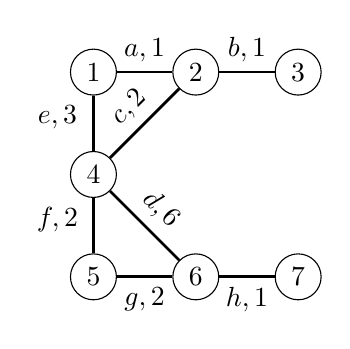
\begin{tikzpicture}
            \tikzset{Vertex/.style={%
                    shape=circle,%
                    draw=black,%
                    minimum size=10pt,%
                    radius=1cm,%
                    inner sep=3pt,%
                    node distance=1.3cm,%
                }}
        
                \node[Vertex] (1) {$1$};
                \node[Vertex, right of=1] (2) {$2$};
                \node[Vertex, right of=2] (3) {$3$};
                \node[Vertex, below of=1] (4) {$4$};
                \node[Vertex, below of=4] (5) {$5$};
                \node[Vertex, right of=5] (6) {$6$};
                \node[Vertex, right of=6] (7) {$7$};
        
                \path (1) edge[-,line width=1pt] node[above]{$a,1$} (2);
                \path (2) edge[-,line width=1pt] node[above]{$b,1$} (3);
                \path (4) edge[-,line width=1pt] node[above,sloped]{$c,2$} (2);
                \path (4) edge[-,line width=1pt] node[above,sloped]{$d,6$} (6);
                \path (4) edge[-,line width=1pt] node[above,xshift=-13pt,yshift=-6pt]{$e,3$} (1);
                \path (4) edge[-,line width=1pt] node[above,xshift=-13pt, yshift=-6pt]{$f,2$} (5);
                \path (5) edge[-,line width=1pt] node[below]{$g,2$} (6);
                \path (6) edge[-,line width=1pt] node[below]{$h,1$} (7);
        \end{tikzpicture}%
        \begin{center}%
            \vspace{-12pt}%
            $(s,t) = (2, 6)$%
        \end{center}
    \end{minipage}\hfill%
    \begin{minipage}{0.50\textwidth}
        \begin{center}
            \begin{minipage}{1.0\textwidth}
                \begin{minipage}{0.5\textwidth}
                    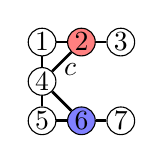
\begin{tikzpicture}
                        \tikzset{Vertex/.style={%
                                shape=circle,%
                                draw=black,%
                                minimum size=10pt,%
                                inner sep=0pt,%
                                node distance=0.5cm,%
                            }}
                    
                            \node[Vertex] (1) {$1$};
                            \node[Vertex, fill=red!50, right of=1] (2) {$2$};
                            \node[Vertex, right of=2] (3) {$3$};
                            \node[Vertex, below of=1] (4) {$4$};
                            \node[Vertex, below of=4] (5) {$5$};
                            \node[Vertex, fill=blue!50, right of=5] (6) {$6$};
                            \node[Vertex, right of=6] (7) {$7$};
                    
                            \path (1) edge[-,line width=1pt] (2);
                            \path (2) edge[-,line width=1pt] (3);
                            \path (4) edge[-,line width=1pt] node[xshift=3pt, yshift=3pt, below]{$c$} (2);
                            \path (4) edge[-,line width=1pt] (6);
                            \path (4) edge[-,line width=1pt] (1);
                            \path (4) edge[-,line width=1pt] (5);
                            \path (5) edge[-,line width=1pt] (6);
                            \path (6) edge[-,line width=1pt] (7);
                    \end{tikzpicture}
                \end{minipage}\hfill%
                \begin{minipage}{0.5\textwidth}
                    $CPD[2,6] = c$
                \end{minipage}

                \begin{minipage}{0.5\textwidth}
                    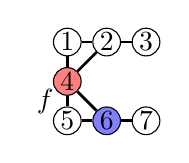
\begin{tikzpicture}
                        \tikzset{Vertex/.style={%
                                shape=circle,%
                                draw=black,%
                                minimum size=10pt,%
                                inner sep=0pt,%
                                node distance=0.5cm,%
                            }}
                    
                            \node[Vertex] (1) {$1$};
                            \node[Vertex, right of=1] (2) {$2$};
                            \node[Vertex, right of=2] (3) {$3$};
                            \node[Vertex, fill=red!50, below of=1] (4) {$4$};
                            \node[Vertex, below of=4] (5) {$5$};
                            \node[Vertex, fill=blue!50, right of=5] (6) {$6$};
                            \node[Vertex, right of=6] (7) {$7$};
                    
                            \path (1) edge[-,line width=1pt] (2);
                            \path (2) edge[-,line width=1pt] (3);
                            \path (4) edge[-,line width=1pt] (2);
                            \path (4) edge[-,line width=1pt] (6);
                            \path (4) edge[-,line width=1pt] (1);
                            \path (4) edge[-,line width=1pt] node[xshift=-8pt]{$f$} (5);
                            \path (5) edge[-,line width=1pt] (6);
                            \path (6) edge[-,line width=1pt] (7);
                    \end{tikzpicture}
                \end{minipage}\hfill%
                \begin{minipage}{0.5\textwidth}
                    $CPD[4,6] = f$
                \end{minipage}

                \begin{minipage}{0.5\textwidth}
                    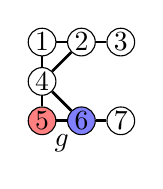
\begin{tikzpicture}
                        \tikzset{Vertex/.style={%
                                shape=circle,%
                                draw=black,%
                                minimum size=10pt,%
                                inner sep=0pt,%
                                node distance=0.5cm,%
                            }}
                    
                            \node[Vertex] (1) {$1$};
                            \node[Vertex, right of=1] (2) {$2$};
                            \node[Vertex, right of=2] (3) {$3$};
                            \node[Vertex, below of=1] (4) {$4$};
                            \node[Vertex, fill=red!50, below of=4] (5) {$5$};
                            \node[Vertex, fill=blue!50, right of=5] (6) {$6$};
                            \node[Vertex, right of=6] (7) {$7$};
                    
                            \path (1) edge[-,line width=1pt] (2);
                            \path (2) edge[-,line width=1pt] (3);
                            \path (4) edge[-,line width=1pt] (2);
                            \path (4) edge[-,line width=1pt] (6);
                            \path (4) edge[-,line width=1pt] (1);
                            \path (4) edge[-,line width=1pt] (5);
                            \path (5) edge[-,line width=1pt] node[yshift=-8pt]{$g$} (6);
                            \path (6) edge[-,line width=1pt] (7);
                    \end{tikzpicture}
                \end{minipage}\hfill%
                \begin{minipage}{0.5\textwidth}
                    $CPD[5,6] = g$
                \end{minipage}
            \end{minipage}

        \end{center}     
    \end{minipage}

    \begin{coloredBlock}{\CPDPathName{}}[OliveGreen][white]
        Given a graph $G$, the \CPD{} associated to $G$, a source node $s$ and target node $t$, 
        the $\CPDPath{s}{t}$ is the path generated by iteratively retrieving the first optimal move from the \CPD{} followed by the update

        With \CPD{}, given a graph and a target node $t$, any node $n$ has \textbf{implicitly} associated an optimal path to $t$ ($\CPDPath{}[n \rightarrow t]$)
    \end{coloredBlock}

\end{frame}